\chapter{Write Away 3}

\begin{figure}[H]
    \centering
    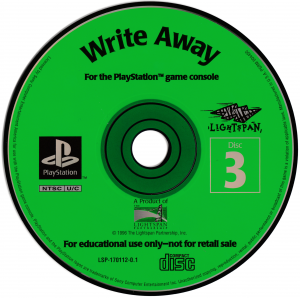
\includegraphics[width=\textwidth/2]{./Games/WriteAway/Images/WriteAway3CD.png}
    \caption{Write Away 3 CD}
\end{figure}

The third of the ten Write Away games published and released by The Lightspan Partnership for the PlayStation 1.

Write Away 3 features nine video programs, including an introduction video, eight story videos, and a conclusion video:

\begin{itemize}
    \item Write Away Episode Three Introduction
    \item Fluffy the Snowman by Doyle Bonaduce
    \item The BunnyThat Cried by Samantha Anderson (spelling mistake in the title of the video)
    \item Wild Wyoming by Charles Barryman \& Ansley Stewart
    \item Pizza by Greg Hernandez
    \item Halloween Mystery by Julie Chen
    \item The Boy and the Alien by Brandon Walker
    \item The Bossy Princess by Chris Jackson
    \item Obtuse Man and Square Boy by Ryan Hammond
    \item Write Away Conclusion
\end{itemize}

\clearpage
\newpage

\section{Transcription}

\subsection{Fluffy the Snowman by Doyle Bonaduce}

SCOUT:
Brian, why are you dressed like that?

BRIAN:
I'm waiting for my favorite time of year - winter.
With the snow.
Lots of snow.
I love snow.

SCOUT:
Well, since you can't wait for winter, I found a great story where the author puts you in a wintry mood with his main character, a lonely Snowman.
This next story comes to us from Doyle Bonaduce, a first-grader from Town Point Elementary.
Watch with us as we meet a very interesting character in Fluffy the Snowman.

SCOUT (VOICE OVER):
Once upon a time, there was a snowman who stood all alone in the snow.
He was a lonely Snowman.

FLUFFY:
I'm so lonely.
I just had somebody to play with.
Look, children!
Maybe they'll let me play with them.
Can I play with you? Hi.

CHILDREN:
Yes, sure.

SCOUT (VOICE OVER):
Fluffy played with his new friends until nighttime when they all went home to go to sleep.

CHILDREN:
Bye Fluffy!

FLUFFY:
See you tomorrow!

SCOUT (VOICE OVER):
And left Fluffy all alone again.

FLUFFY:
Bye, kids!
It's great to have friends.

SCOUT (VOICE OVER):
The next morning, the sun was shining.

FLUFFY:
Hi Mr. Sun.
I can't wait for my new friends to come out.

SUN:
Yeah cool.

FLUFFY:
It's sure getting warm.

SCOUT (VOICE OVER):
Finally, the children came out to play with Fluffy, but Fluffy wasn't there.

CHILD 1:
Oh no, poor Fluffy melted.

SUN:
What?

CHILD 2:
Will he come back next year?

FLUFFY:
He he he.

CHILD 1:
I'm sure he will.

FLUFFY:
He he he.

\subsection{The Bunny That Cried by Samantha Anderson}

PAUL:
Here fishy, here's some food.
You know, when I look at my fish in there, swimming all by himself, I wonder what he's thinking.
Is he happy?
Is he sad?
Maybe he'd even like a fish friend.
Then I start thinking about all kinds of animals.
Do they have feelings?
Do they have love and loneliness?
As a writer, when you give human emotions to animals, it's called personification.
Oh boy, that's a big word, but it opens a whole world of creativity when you put your thoughts down on paper.
Well, I guess my question about animals having human emotions is answered by Samantha Anderson from Harris Elementary in "The Bunny That Cried."

BUNNY1 :
Dear diary, I have a buddy.
A buddy who cries out, 'I want a friend,' but the only animals that come to visit me are worms.
All they ever ask is -

WORMS:
Got any dirt?

BUNNY1 :
And all they ever want to do is play 'Slime Around the Rosie.'

WORMS:
Slime around the Rosie,
we're slimy and we're nosy,
dirt clods, dirt clods, we all crawl down.

BUNNY1 :
So, I cry out, 'Attention please, I'm lonely. Rabbits only!'

WORM 1:
How rude!

WORM 2:
Boring!

WORM 1:
Let's go.

WORM 2:
Okay.

BUNNY1 :
That's when I heard something in the Cabbage Garden.
Who's out there?
Don't hurt me, please!
But that's when I noticed that there were two bunny ears just like mine.
It was a new bunny friend I've been waiting for.
Then we both yelled -

BUNNY 1, BUNNY 2:
Hey world!
I've got a friend now!

BUNNY 1:
And so, now I'll close dear diary, because I had to play with my new friend.

\subsection{Wild Wyoming by Charles Barryman \& Ansley Stewart}

JOE:
[don't know what he's saying]

BRIAN:
Hey, let's go, we're ready for the next story.

JOE:
Oh, I'm sorry, um, enough of that crying stuff.
Our next story takes place where men are men and cows are cows and mountains are mountains.

BRIAN:
Joe, come on.

JOE:
Ah, I'm sorry.
I'm just really excited about this next story.
Watch what happens when two authors come together and make one great adventure story.
It comes to us from kindergartener Charles Berryman and fourth-grader Ansley Stewart from Alps Road School.
Now, let's watch 'Wild Wyoming'.
Yeehaw!

WILLIAM:
Hi, I'm William, and this is my friend Ainsley.
We're going to Wyoming for our summer vacation to study the Wild West.
Right, Ainsley?

AINSLEY:
Right, and I sure hope it's wild.

WILLIAM:
Yeah

AINSLEY:
Come on.

WILLIAM:
Let's go.

WILLIAM (VOICE OVER):
On our plane ride, we went through a thunderstorm, and it was pretty rough.
Finally, we got to Wyoming, and my Uncle Bill was waiting for us to take us to his house.

UNCLE BILL:
Well kids, it's good to have you here.
Tomorrow, we'll go exploring. Come on, let's go home.

WILLIAM (VOICE OVER):
While we were unpacking, we found something.

AINSLEY:
Hey, what's that under the bed?
Look, it's a treasure map.

WILLIAM:
I wonder if it's real.
Let's ask Uncle Bill.
Uncle Bill, Uncle Bill!

UNCLE BILL:
[Yep]

WILLIAM:
Look, we found a map.

UNCLE BILL:
Uh! This is a real treasure map.
And do you know how I know?

AINSLEY, WILLIAM:
How?

UNCLE BILL:
It says 'Real Treasure Map' right there.
Ha ha ha.
Come on, let's go find some treasure.

WILLIAM:
Yeah.

WILLIAM (VOICE OVER):
We saddled up on some horses and rode on and on, until we found a good place for a campsite.
Lucky for us, Uncle Bill brought a cellular phone to call the weatherman to see what the weather would be like.

UNCLE BILL:
Well, kids, there's a sandstorm on the way.
But don't worry, we're going to be safe.
Now, go to sleep.
Pleasant dreams.

WILLIAM (VOICE OVER):
The next day, we rode, following the map, when suddenly, we found two kids that were lost.

GIRL:
Help help!
We got lost in the sandstorm.

BOY:
Now we can't find a way back.
Please help us.

UNCLE BILL:
Well, of course.
Hey, hey, we're looking for treasure.
Come on with us.

BOY, GIRL:
Okay.

WILLIAM:
Let's look on the map, Uncle Bill, to find OUR treasure.

AINSLEY:
Now look, it says according to this map that the gold should be right over there in that gold mine.
Right where that big, nasty bull is standing.

UNCLE BILL:
Don't worry kids.
I'll distract him while you go on the mine.
Toro. Toro.

WILLIAM (VOICE OVER):
Christy and I ran ahead, but we tripped.
Luckily, we landed right on a pile of gold.
We grabbed all we could and ran back to show Uncle Bill and the others.

UNCLE BILL:
That's it, you stay away, you nasty bull.

WILLIAM:
Uncle Bill, look, we found gold!
Is it real, Uncle Bill?"

UNCLE BILL:
Hey, let me see, I'll taste it.
That ain't real gold - it's Fool's Gold.

WILLIAM, AINSLEY, BOY, GIRL:
Augh.

UNCLE BILL:
Hey that's all right.
We had a mighty fine adventure, didn't we?

WILLIAM, AINSLEY, BOY, GIRL:
Yeah!

UNCLE BILL:
Let's go home and have ourselves a barbecue.

WILLIAM, AINSLEY, BOY, GIRL:
Yeah!

EVERYONE:
Aah! Aah! Aah!
Yeehaw!
The end.

BULL:
He he he.

\subsection{Pizza by Greg Hernandez}

SCOUT:
I can't decide what to order, everything looks so good.

PAUL:
There are so many choices.

TRESSY:
I could get that? Yes? No?

JOE:
Or maybe that?

BRIAN:
You know, the same thing happens to me when I'm writing a story.
I have so many ideas, I can't decide which one's the best.
This happens to everybody when they write, but you have to make a choice.
Fifth-grader Greg Hernandez from Washington Elementary sure does IN his poem entitled "Pizza".

PIZZA SERVER:
Welcome totally excellent dudes to\dots Pizza City, yeah!
Can I like, take your orders?

WOMAN 1:
I would like a pizza please, with lots and lots and lots of cheese.

MAN 1:
Give me all you got of Ham and lots and lots and lots of spam.

WOMAN 2:
Olives, sausage, peppers too.
Tomatoes well just a few.

MAN 2:
Give me tons of anchovies and put them underneath the cheese.

WOMAN 1:
Give me all you've got of sauce, I don't care how much it costs.

MAN 1:
Now put on some pepperoni, and we don't want no stinking baloney.

WOMAN 2:
Pineapple will top it all, eating it will be a ball.
Wee!

MAN 2:
Don't forget Canadian bacon.

PIZZA SERVER:
Sorry, dude, but it's all taken.

WOMAN 1, WOMAN 2, MAN 1, MAN 2:
What?

PIZZA SERVER:
Whoa dudes, just kidding.

WOMAN 1, WOMAN 2, MAN 1, MAN 2:
Woah?
Pizza\dots
The end.

\subsection{Halloween Mystery by Julie Chen}

NARRATOR 1:
And now, welcome to another spine-tingling Tales From The Script: A Halloween Mystery.

PAUL:
Hello, my little ghouls and ghoulettes!
There's nothing I like more than Halloweens stories full of fright.
Oh, and so does she.
I found a terrifyingly scary story that takes place at a fun little Halloween party where the guests may not be as they seem.
It comes from third-grader Julie Chen of Handy Elementary.
Now, let's watch as anything can happen in "The Halloween Mystery."

NARRATOR 2:
Vinnie Valvano was at a costume party on Halloween night.
Everyone was dancing and having a great time.

VINNIE:
Hey Betsy?

BETSY:
Huh.

VINNIE:
Who's that in that dinosaur costume?

BETSY:
I don't know. Look how he's dancing!

NARRATOR 2:
Soon, the party was over, and everyone went home.
Everyone, that is, except for Vinnie and the dinosaur.

VINNIE:
Oh, I guess my Dad forgot to pick me up.
Better walk home now.

NARRATOR 2:
Vinnie began to walk home the only way he could, down a dark, dreary dirt road where the trees seemed to be staring at him.

TREE 1:
Psst!
Hey kid!
You one of those kids that likes toothpicks?

TREE 2:
Kid.
You don't like log cabins, do you?

TREE 1:
Bet he does.

TREE 2:
I bet he does.

TREE 1:
Bet he does.

TREE 2:
I bet he does.

VINNIE:
Aah!

NARRATOR 2:
Vinnie continued to walk down the road but stopped suddenly.
He heard footsteps behind him.
He turned around to look and saw the dinosaur from the party.
The dinosaur was coming closer and closer.
Then he started running until he heard the dinosaur call out -

DINOSAUR:
Vinnie! Vinnie!

VINNIE:
He knows my name!
Aah!

NARRATOR 2:
The dinosaur took off his head and said,

DAD:
Vinnie, what were you running for?
I wanted to drive you home.

VINNIE:
Dad, what are you doing in that dinosaur costume?

DAD:
Oh, Betsy's parents called and asked me to help chaperone her party.
Neat costume, huh?

VINNIE:
Yeah.

DAD:
I really scared you.
I'm sorry, son.

VINNIE:
Oh me, scared? I'm not scared of anything.

GHOUL (VOICE):
Ooooh!

DAD:
Let's go home, son.

PAUL:
Well, I don't know about you, but I'll never go walking alone on Halloween night again.
Is my friend into something extinct?
Well, I've got to go now, but people's ghoulishly good stories are coming my way, and I'll see you next time on Tales From The Script.

\subsection{The Boy and the Alien by Brandon Walker}

SCOUT:
Do you ever wonder if there's life on other planets?
I do.
I wonder if we could be friends with other beings.
After all, love and friendship is what make the world, our worlds, go round.
And writing your feelings down on paper is a great way of expressing them with other people, and that's exactly what this next author did.
First-grader Brandon Walker from Midland School explores his feelings in his wonderful story "The Boy and the Alien."

NARRATOR:
Once there was a boy named Brandon who loved to play his harmonica.
One day, as he was walking, he found a box.

BRANDON:
Wow, look!
Someone must have lost their box.
Oh well, I'll take it home with me.

NARRATOR:
What Brandon didn't know was that this was a magic box.
If you drew on it, it would change into the picture you drew.

BRANDON:
Think I'll draw a spaceship on the side of this box, because I love space.

LAUNCH CONTROLLER:
We have main engine ignition!

NARRATOR:
Suddenly, Brandon's room turned into a spaceship, and he flew up to the planet Pluto.

BRANDON:
This is amazing! I'm gonna go explore.

NARRATOR:
Brandon was walking when suddenly he saw an alien.

IZZY:
Ni ni na ni no ni nee.

NARRATOR:
At first, Brandon was frightened.

BRANDON:
Don't hurt me!

NARRATOR:
But Brandon soon learned that the alien was friendly.

BRANDON:
Thanks! I'm Brandon.
I'm from Earth.

IZZY:
Izzy.
Friend.

NARRATOR:
The alien showed Brandon an unusual necklace she had.

BRANDON:
That's neat!

IZZY:
Here, you can have it.
When you want to talk to me, just wear it.
We can talk anytime.

BRANDON:
Here, I want you to have my harmonica.
Whenever you play it, I'll hear the music.

NARRATOR:
They hugged and said goodbye.
Then Brandon went back home.

BRANDON:
Bye, Izzy!

IZZY:
Bye!

NARRATOR:
Back at home, Brandon often used the special necklace to talk to Izzy, and Izzy would play music on the harmonica for Brandon to hear.

BRANDON:
I learned that wherever I go, I can make new friends, even if we are different.

IZZY:
Ni ni na ni no ni noo.

NARRATOR:
And Brandon and Izzy remain friends forever.
The end.

\subsection{The Bossy Princess by Chris Jackson}

BRIAN:
Oh hi.
I just finished the ending on the story I wrote.
For the third time.
I can't make up my mind if my ending should be happy or sad, or, or both.
Most endings are "happily ever after," but I like it when a writer can add a new twist to an old story and surprise you with a very unusual ending.
Chris Jackson from Lakeview School does just that when he takes us to the wacky Kingdom of "The Bossy Princess."

BRIAN (VOICE OVER):
Once upon a time, there lived a princess.
Now, she was very pretty, but she was also very bossy.

PRINCESS:
Where's my new dress?
Where's my lunch?
Why won't they hurry, hurry, hurry?

BRIAN (VOICE OVER):
When she did not get what she wanted, she would have a fit and scream.
This made her father, the king, very unhappy.

KING:
Why must my daughter be so bossy?
We should be more appreciative of what she has.
I know, perhaps seeing the handsome prince will help her.

PRINCE:
Good morning, sweet princess.
How lovely you look today.

PRINCESS:
Really?
Get me my mirror!
No, not that one, that one.
Yeah, that one right there. Give it to me!
Please, get out of my sight!

BRIAN (VOICE OVER):
Meanwhile, in the enchanted part of the forest, the evil witch was planning to take over the kingdom.

WITCH:
There.
The ransom note is finished.
In order to take over the kingdom, I will kidnap the princess.
The king will be so upset - he will give me the kingdom in exchange for his daughter.
Then I will be the most powerful witch in the kingdom.
Now for a disguise.

BRIAN (VOICE OVER):
And so the witch disguised herself as a fortune teller and went to the castle.
Meanwhile, at the castle, the bossy princess sat reading her favorite book.

WITCH:
Hello pretty princess.
Have your fortune told?

PRINCESS:
Oh, yes, sit down.
Here you go, start with my lifeline.
No, start with my love line.

WITCH:
You will take a short journey with a stranger.
Be in danger?
And I will take over the kingdom!

BRIAN (VOICE OVER):
The witch kidnapped the princess and left a ransom note.
The prince heard the scream and came running, but the princess was gone.
He saw a note and gave it to the king.

PRINCE:
Your highness, the evil witch has kidnapped the princess.
We must save her!

KING:
We must?
Oh, of course, we must.
Yes, yes, go save her my son.
Oh, all right, I'll go too.

BRIAN (VOICE OVER):
Back at the witch's castle, the princess was bossing the evil witch around.

PRINCESS:
Hey you, yeah you!
I'm thirsty.
I want some water, and none of this tap stuff.
I want bottled water.
And listen, you have to untie these ropes.
I'm swelling up like a balloon.

WITCH:
Oh, please stop it!
Just can't take it anymore.
Just, just go home!

BRIAN (VOICE OVER):
The witch finally let the princess go.

PRINCE:
Princess, there you are!
I looked everywhere for you.
Everybody's been so worried about you.

PRINCESS:
They have?

KING:
Uh, yes, we have.

PRINCESS:
Would you marry me?

KING:
Yes you will.

PRINCESS:
Yes, but first, there are a few rules we'll have to talk about before we get married.

BRIAN (VOICE OVER):
And so the princess and the prince lived unhappily ever after.

WITCH:
Oh no, they didn't!
Ibby bobby ossy, this princess is no longer bossy.

PRINCESS:
And like I was saying, I think you're wonderful, and I promise never to be bossy again.

WITCH:
Hey there, handsome.
Wanna go to a wedding?
Who says fairy tales don't have happy endings?

BRIAN (VOICE OVER):
And that is how they all lived happily ever after.
The bossy princessl
The end.

\subsection{Obtuse Man and Square Boy by Ryan Hammond}

TRESSY:
Now I will save the world from the evil powers beyond!
It's rays are great, but I can hold them back!
Oh hi!
I was just pretending I'm a superhero.
Sometimes I like to pretend I'm a cowgirl.
Well, howdy partner!
Sometimes I like to pretend I'm a nurse.
Open wide, please!
With my imagination, I can be anything or anyone I want to be, and it helps in my creative writing too.
There are no limitations on who or what I write about, and there's no limitation in plot or character in this next story.
It's written by sixth-grader Ryan Hammond from Wildomar Elementary.
Watch as two unlikely superheroes save the day in 'Obtuse Man and Square Boy'!

TRESSY (VOICE OVER):
Mardi Gras and Et Cetera dreamed of being superheroes.

MARDY GRAS:
Gosh, if only I could fly like Superman.

ED CETERA:
Yeah, and if only I had the strength of The Incredible Hulk.

TRESSY (VOICE OVER):
This dream unfortunately became a reality when a terrible mistake occurred.
Arch Enemy of the world, Really Naughty Man, had just completed his experiment and was ready to test it.

REALLY NAUGHTY MAN:
My experiment is spreading!
I've created the ultimate weapon [that] take over the whole world!
Thunder clouds filled with stupid rain.
When it rains on everybody, they will become stupid, and I will be ruler over all that is stupid!
Oh bad boy, bad boy.
Ha ha ha!

TRESSY (VOICE OVER):
Really Naughty Man released the clouds, but they only gathered over Marty and Ed's house.
It rained and rained on Marty and Ed, and it made them stupid.
But it also turned them into their traditional comic book heroes with X-ray vision.

MARTY GRAS (OBTUSE MAN):
So that's where that sock went!

TRESSY (VOICE OVER):
Super strength.
Invunerability to their enemy.
The ability to fly!
And the greatest power of all\dots

MARTY GRAS (OBTUSE MAN):
Knowing what's on TV without turning it on!
I will be Obtuse Man, and my job will be to watch TV with my trusty channel changer!

ED CETERA (SQUARE BOY):
And I will be Square Boy.
And, as your faithful sidekick, I will work at Burger World to ensure the public quality fast food!

TRESSY (VOICE OVER):
Really Naughty Man saw that his plan had not worked, and he was mad.

REALLY NAUGHTY MAN:
This isn't gonna stop me!
I'm still gonna take over the world, and I know just how to do it!

TRESSY (VOICE OVER):
As Obtuse Man watched TV, a news flash came on.

NEWS PRESENTER:
This just in.
Really Naughty Man has just announced from his Mega plane that he is taking over the world, and no one can stop him, not even Obtuse Man or Square Boy.
So don't even try!
Everyone, please, do not panic!
Do not panic!
Everything is under control!

MARTY GRAS (OBTUSE MAN):
Oh no!
I must save the world!
Thank goodness for my trusty VCR.
Now I won't miss Gilligan's Island.
And now to get Square Boy!

ED CETERA (SQUARE BOY):
Welcome to Burger World, may I help you?

CUSTOMER:
*inaudible*

ED CETERA (SQUARE BOY):
I'm sorry, you'll have to speak up.
I can't understand a word that you are saying and -

MARTY GRAS (OBTUSE MAN):
Square Boy!
Come, Really Naughty Man is at it again.
It's time to save the world!

ED CETERA (SQUARE BOY):
Yes!

REALLY NAUGHTY MAN:
Hello world, this is Really Naughty Man in my mega plane, and I'm gonna drop my stupid brain if you don't give up!

MARTY GRAS (OBTUSE MAN):
Your days of naughtiness are over!
Whoa, watch the propeller, Square Boy!

ED CETERA (SQUARE BOY):
you've been a very naughty man!
Now give up, you're surrounded!

REALLY NAUGHTY MAN:
Never, never!
Uh oh... I run out of gas.
All right, I surrender.
Oh you're just too much for me.

TRESSY (VOICE OVER):
Later that day, Obtuse Man and Square Boy gave Really Naughty Man his punishment.

MARTY GRAS (OBTUSE MAN):
You must write 'I will not try to conquer the world' 2,000 times.

REALLY NAUGHTY MAN:
Done, and I've learned a valuable lesson.

MARTY GRAS (OBTUSE MAN), ED CETERA (SQUARE BOY):
What's that?

REALLY NAUGHTY MAN:
Never try to conquer the world on a half a tank of gas.
I'm out of here, see ya!

TRESSY (VOICE OVER):
And so Marty and Ed truly were superheroes, and they had saved the day!

REALLY NAUGHTY MAN:
For now...

\subsection{Write Away Conclusion}

TRESSY:
Well, we hope you enjoyed watching the stories today as much as we did presenting them.

PAUL:
I can't wait to see what you write for our next show.

TRESSY:
That's right, you've already shown us what good writers you are, but we need a lot more stories for future shows.

JOE:
Send us more adventure stories.

BRIAN:
More funny stories.

SCOUT:
More romantic stories and poems

PAUL:
More mysteries.

TRESSY:
It doesn't really matter what kind of stories you write, just let your imaginations run free and remember\dots

EVERYONE:
Write away!

\section{Credits}